\let\negthickspace\undefined
\documentclass[journal,12pt,twocolumn]{IEEEtran}
\usepackage{cite}
\usepackage{amsmath,amssymb,amsfonts,amsthm}
\usepackage{algorithmic}
\usepackage{graphicx}
\usepackage{textcomp}
\usepackage{xcolor}
\usepackage{txfonts}
\usepackage{listings}
\usepackage{enumitem}
\usepackage{mathtools}
\usepackage{gensymb}
\usepackage{comment}
\usepackage[breaklinks=true]{hyperref}
\usepackage{tkz-euclide} 
\usepackage{listings}
\usepackage{gvv}                                        
\def\inputGnumericTable{}                                 
\usepackage[latin1]{inputenc}                                
\usepackage{color}                                            
\usepackage{array}                                            
\usepackage{longtable}                                       
\usepackage{calc}                                             
\usepackage{multirow}                                         
\usepackage{hhline}                                           
\usepackage{ifthen}                                           
\usepackage{lscape}
\setlength{\arrayrulewidth}{0.5mm}
\setlength{\tabcolsep}{18pt}
\renewcommand{\arraystretch}{1.5}
\newtheorem{theorem}{Theorem}[section]
\newtheorem{problem}{Problem}
\newtheorem{proposition}{Proposition}[section]
\newtheorem{lemma}{Lemma}[section]
\newtheorem{corollary}[theorem]{Corollary}
\newtheorem{example}{Example}[section]
\newtheorem{definition}[problem]{Definition}
\newcommand{\BEQA}{\begin{eqnarray}}
\newcommand{\EEQA}{\end{eqnarray}}
\newcommand{\define}{\stackrel{\triangle}{=}}
\theoremstyle{remark}
\newtheorem{rem}{Remark}
\begin{document}
\title{Sequence(19) 10.5.3}
\author{EE23BTECH11051-Rajnil Malviya}
\date{January 2024}
\maketitle
\subsection*{\textit{Question :-}}
200 logs are stacked in the following manner: 20 logs in the bottom row, 19 in the next row,
18 in the row next to it and so on . In how many rows are the 200 logs placed
and how many logs are in the top row?

\begin{table}[h!]
   
        \begin{tabular}{ | m{1.0cm} | m{3cm} |m{1cm} |} 
  \hline
 Symbol &Description& Value \\ 
 \hline
$x(0)$&bottom row& 20  \\
\hline
d&common difference & -1  \\
\hline
y\brak n& total number of logs&200 \\
\hline
x\brak n&number of logs in n row&  depends on n\\
\hline
\end{tabular}\\
\caption{}
\label{Table:1}

       
    \end{table}
For an Arithmetic Progression :-
\begin{align}x\brak n=\sbrak {x(0)+n d} u \brak n\\
x\brak n=\sbrak{20-n} u \brak n\\
 X(Z)=\frac{20-21z^{-1}}{(1 - z^{-1})^2}  \quad \abs{ z} > 1\\
y \brak n = x\brak n*u\brak n\\
Y \brak z = X\brak zU\brak z\\\
Y(z) = \frac{20-21z^{-1}}{(1 - z^{-1})^3}\end{align}
 Using Contour Integration to find the inverse $Z$-transform,
\begin{align}
    y(n)&=\frac{1}{2\pi j}\oint_{C}Y(z) \;z^{n-1} \;dz  \\
    &=\frac{1}{2\pi j}\oint_{C} \frac{(20-21z^{-1}) z^{n-1}}{(1 - z^{-1})^3} \;dz 
\end{align}
We can observe that the pole is repeated $3$ times and thus $m=3$,
\begin{align}
    R&=\frac{1}{\brak {m-1}!}\lim\limits_{z\to a}\frac{d^{m-1}}{dz^{m-1}}\brak {{(z-a)}^{m}f\brak z}  \\
    &=\frac{1}{\brak {2}!}\lim\limits_{z\to 1}\frac{d^{2}}{dz^{2}}\brak {20 z^{n+2}-21 z^{n+1}}   \\
    &=\frac{1}{2}\lim\limits_{z\to 1}(20(n+2)(n+1)z^{n}-21(n)(n+1)z^{n-1})   \\
    &=\frac{1}{2}[20(n+2)(n+1)-21(n)(n+1)]\end{align}
      \begin{align}
       R &= y\brak n \\
  200 &=\frac{1}{2}\sbrak{20\brak{n+2}\brak{n+1}-21\brak{n}\brak{n+1}}\\
   n &=15\; ,\;24\end{align}
  \begin{align}
 & x\brak{n}>0\end{align}
Using equation 2
\begin{align} &x\brak{15}=5\\
 &x\brak{24}=-4 \end{align}
x\brak{24} is rejected because it is negative
\begin{align}x\brak{15}=5\end{align}
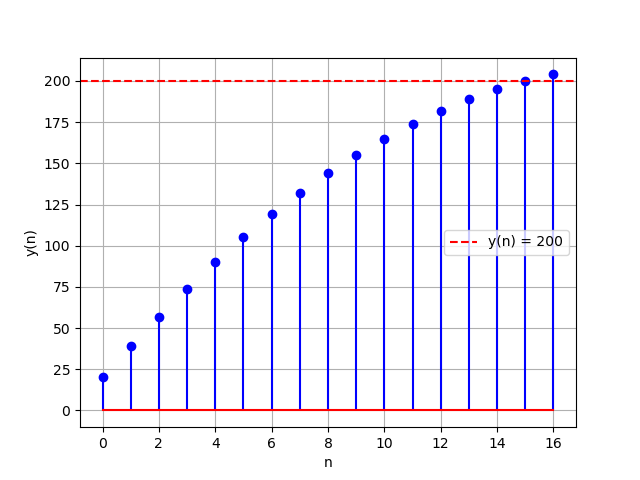
\includegraphics[width=2\linewidth]{figs/f2.png}\\\\

\end{document}
